% This file was created by tikzplotlib v0.9.8.
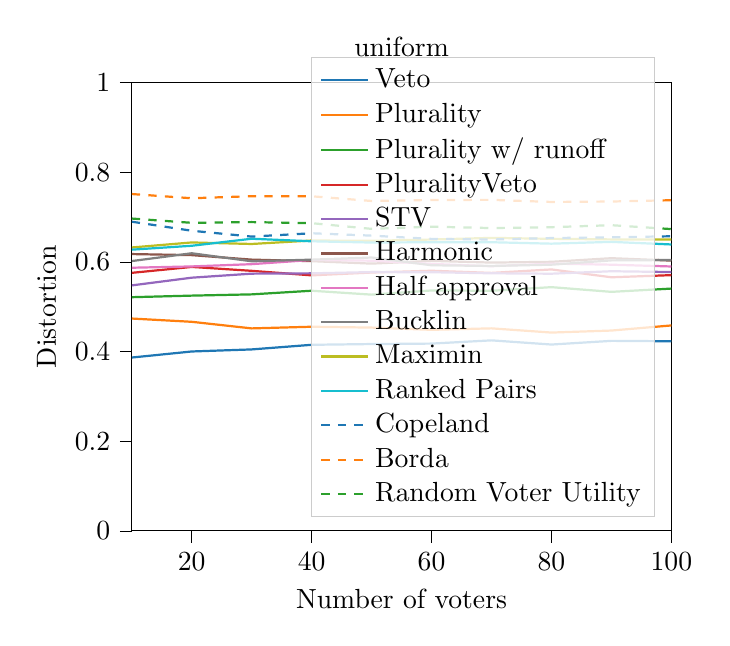
\begin{tikzpicture}

\definecolor{color0}{rgb}{0.12156862745098,0.466666666666667,0.705882352941177}
\definecolor{color1}{rgb}{1,0.498039215686275,0.0549019607843137}
\definecolor{color2}{rgb}{0.172549019607843,0.627450980392157,0.172549019607843}
\definecolor{color3}{rgb}{0.83921568627451,0.152941176470588,0.156862745098039}
\definecolor{color4}{rgb}{0.580392156862745,0.403921568627451,0.741176470588235}
\definecolor{color5}{rgb}{0.549019607843137,0.337254901960784,0.294117647058824}
\definecolor{color6}{rgb}{0.890196078431372,0.466666666666667,0.76078431372549}
\definecolor{color7}{rgb}{0.737254901960784,0.741176470588235,0.133333333333333}
\definecolor{color8}{rgb}{0.0901960784313725,0.745098039215686,0.811764705882353}

\begin{axis}[
legend cell align={left},
legend style={
  fill opacity=0.8,
  draw opacity=1,
  text opacity=1,
  at={(0.97,0.03)},
  anchor=south east,
  draw=white!80!black
},
tick align=outside,
tick pos=left,
title={uniform},
x grid style={white!69.0196078431373!black},
xlabel={Number of voters},
xmin=10, xmax=100,
xtick style={color=black},
y grid style={white!69.0196078431373!black},
ylabel={Distortion},
ymin=0, ymax=1,
ytick style={color=black}
]
\addplot [thick, color0]
table {%
10 0.3865
20 0.4
30 0.4046
40 0.4149
50 0.4166
60 0.4176
70 0.4248
80 0.4155
90 0.4237
100 0.4228
};
\addlegendentry{Veto}
\addplot [thick, color1]
table {%
10 0.4735
20 0.4662
30 0.4515
40 0.4552
50 0.4533
60 0.4483
70 0.4516
80 0.4422
90 0.4467
100 0.4581
};
\addlegendentry{Plurality}
\addplot [thick, color2]
table {%
10 0.5211
20 0.5246
30 0.5274
40 0.5355
50 0.5268
60 0.5361
70 0.5355
80 0.5435
90 0.533
100 0.5403
};
\addlegendentry{Plurality w/ runoff}
\addplot [thick, color3]
table {%
10 0.5754
20 0.5886
30 0.5799
40 0.5698
50 0.5761
60 0.5801
70 0.5753
80 0.583
90 0.5655
100 0.5703
};
\addlegendentry{PluralityVeto}
\addplot [thick, color4]
table {%
10 0.5474
20 0.5646
30 0.5736
40 0.5743
50 0.5771
60 0.5768
70 0.5744
80 0.5735
90 0.579
100 0.5772
};
\addlegendentry{STV}
\addplot [thick, color5]
table {%
10 0.6173
20 0.6149
30 0.6049
40 0.6015
50 0.596
60 0.6021
70 0.5983
80 0.6
90 0.6081
100 0.6027
};
\addlegendentry{Harmonic}
\addplot [thick, color6]
table {%
10 0.5868
20 0.5897
30 0.5948
40 0.6041
50 0.6025
60 0.5954
70 0.5901
80 0.596
90 0.5936
100 0.5896
};
\addlegendentry{Half approval}
\addplot [thick, white!49.8039215686275!black]
table {%
10 0.6017
20 0.6191
30 0.6012
40 0.6048
50 0.6096
60 0.5923
70 0.5908
80 0.5936
90 0.6032
100 0.604
};
\addlegendentry{Bucklin}
\addplot [thick, color7]
table {%
10 0.632
20 0.6432
30 0.6398
40 0.6475
50 0.6469
60 0.6497
70 0.6534
80 0.6513
90 0.65
100 0.65
};
\addlegendentry{Maximin}
\addplot [thick, color8]
table {%
10 0.6271
20 0.6358
30 0.6515
40 0.6458
50 0.643
60 0.6437
70 0.6437
80 0.6405
90 0.6445
100 0.6387
};
\addlegendentry{Ranked Pairs}
\addplot [thick, color0, dashed]
table {%
10 0.6895
20 0.6693
30 0.6563
40 0.6637
50 0.6584
60 0.6511
70 0.6498
80 0.653
90 0.6547
100 0.657
};
\addlegendentry{Copeland}
\addplot [thick, color1, dashed]
table {%
10 0.7512
20 0.7418
30 0.7464
40 0.7462
50 0.7357
60 0.738
70 0.7382
80 0.7335
90 0.7345
100 0.7374
};
\addlegendentry{Borda}
\addplot [thick, color2, dashed]
table {%
10 0.6965
20 0.687
30 0.6886
40 0.6862
50 0.6735
60 0.6784
70 0.6753
80 0.6772
90 0.6817
100 0.673
};
\addlegendentry{Random Voter Utility}
\end{axis}

\end{tikzpicture}
